\chapter{Implementation} % Main chapter title

\label{Chapter3} % For referencing the chapter elsewhere, use \ref{Chapter1} 

In this chapter, the approaches used in this research is examined. First, the dataset taken from Spotify is mentioned. After that, the three algorithms and the evaluation metrics are discussed in detail.

\section{Dataset}

The dataset for this thesis is a combination between two databases from two services: last.fm \footnote{https://last.fm} and Spotify Web Api \footnote{https://developer.spotify.com/web-api}. First, a list of user, the album they listen, the artists, and the number of times they listen to the album is taken from last.fm. The album name and artist name are then used to get album tracks, which are all the tracks contain in that album, on Spotify. Finally, using the track id of each tracks, track audio features are crawled. 


In the data processing phase, I recognize that some albums have only 1 or 2 tracks. This phenomenon might be due to the lack of data, or because the creators of those albums decide so. However, as an album with just few tracks might not be a good representation for the album, I decide to eliminate all albums that have less than 5 tracks, as following the \textit{Chart Rule} from Official UK Singles Chart \cite{chartUK2017}. Then, for each album, the mean of the acoustic features is calculated, which represents the acoustic features of the whole album. 

The ultimate dataset, creating by joining the mention above databases, contains about 185000 users listening to 64000 different albums. The distribution of user listening is shown in the figure \ref{fig:user_distribution}. In number, the total number of user listening to less than 20 albums accounts for 65\%. The number of user listening to between 20 and 40 albums acquire 19\%. The rest 16\% is accumulated unevenly from user listening to 40 up to 600 albums. 

\begin{figure}[h]
\centering
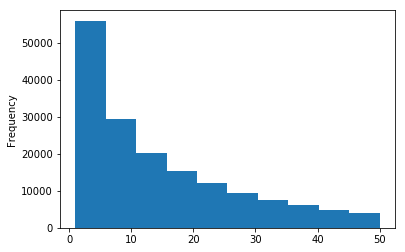
\includegraphics{user_distribution}
\caption{distribution of user listening to less than 50 albums}
\label{fig:user_distribution}
\end{figure}

The final dataset contains the following fields:

\begin{itemize}
\item[•] Username: The user who listen to the album, taken from last.fm database.
\item[•] Album: The name of the album the user listens to.
\item[•] Artist: The artist who performs the album.
\item[•] Playcount: The total number of time the user listens to the album.
\item[•] Energy: A perceptual measurement of intensity and activity in a range from 0 to 1. The higher the score, the higher the energy the track contains. For example, metal rock has high energy, while a Bach prelude is perceived to have low energy. This measurement is built on top of dynamic range, loudness, timbral, onset rate, and general entropy.
\item[•] Speechiness: A measurement of how much spoken words is present compare to music. A value from 0.66 to 1 indicates that the track is mostly spoken words, such as talk show or audio book. Vice versa, a value between 0.33 and 0.66 implies that the track contains both music and speech, ranging from pop to rap music. A value below 0.33 indicates a non speech track. 
\item[•] Acousticness: A evaluation of how much acoustic a track contains compare to how much electronic. Again, a value closer to 1 implements that the track is played with mostly acoustic instruments, such as guitar and harmonica; while a value closer to 0 implements the present of electronic instruments.
\item[•] Danceability: A measurement of how suitable a track is for dancing based on a combination of musical elements including tempo, rhythm stability,  beat strength, and overall regularity. The higher the value, the more danceable the track.
\item[•] Tempo: The overall estimated tempo of a track, measuring in beats per minute (BPM).
\item[•] Instrumentalness: The assessment of how much a track incorporates vocals. The higher the instrumentalness, the greater likelihood the track contains no vocal content. 
\item[•] Key: The key (tonal center) a track is in. Integers map to pitches using Pitch Class notation \footnote{https://en.wikipedia.org/wiki/Pitch\_class}. 
\item[•] Valence: A measure from 0 to 1 of the positiveness of a track. Tracks with high valence sound more positive (e.g. happy, cheerful), and vice versa.
\item[•] Liveness: An indication of whether a track is performed live or in studio. The higher the liveness, the higher possibility that the track is performed live.
\item[•] Loudness: The overall loudness of a track in decibels (dB), with range from -60 to 0 db. 
\end{itemize}

\noindent As some of the features (e.g. key, duration) are not in the scale from 0 to 1, a standardization is necessary to eliminate over-weighting variables. The standardization for all the acoustic features is achieve by subtracting the mean following by dividing by the standard deviation for each feature. 

\section{Algorithms}

The following sections describe my implementation of the three algorithms: a pure collaborative filtering, a pure content-based filtering, followed by the details of the hybrid approach.

\subsection{Pure Collaborative Filtering}
As the number of song outnumbers the number of user, I decide to implement the user-user based collaborative filtering. The algorithm can be summarized in the following steps:

\begin{enumerate}
	\item Calculate similarity between users as Pearson correlation between users' rating vectors. 
	\item For each user, form a neighborhood of \textit{n} users that have the highest similarity.
	\item Compute a prediction for an item from a weighted combination of selected neighbor's ratings. 
\end{enumerate}

In step 3, predictions are calculated using the weighted average of deviations from neighbors' mean. The formula is as follow:

\begin{displaymath}
p_{a,i} = \overline{r}_a + \frac{\sum_{u=1}^{n} (r_{u,i} - \overline{r}_{u}) \times P_{a,u}}{\sum_{u=1}^{n} P_{a,u}}  \tag{1} \label{eq:1}
\end{displaymath}

with \(p_{a,i} \) is the prediction of item i for user a, \(P_{a,i}\) is the similarity between user a and user u, and \(\overline{r}_a\) is the average of the ratings of user a.  

\subsection{Pure Content-based Filtering}
Regression approach is applied to predict user-rating for the content-based filtering method, as linear predictors are proved to be useful when data is high-dimensional \cite{dekel2016linear}. Particularly, the \textit{Stochastic Gradient Descent} algorithm will be used to train the predictors. The formalization of the problem and the algorithm are as follows:

\subsubsection{Problem formalization}
Let \({(x_i, y_i)}_{i=1}^{m}\) be the training set of rating, where each \(x_i \in \mathbb{R}^n\) is an acoustic feature vector and \(y_i \in \mathbb{R} \) is its corresponding user rating. We also define a loss function \( \ell : \mathbb{R}^2 \rightarrowtail \mathbb{R}\) over pairs of label, where \( \ell(p,y) \) is the penalty associating with predicting rating p when the correct rating is y. Depends on the type of loss function, the problem can become a regression problem or a binary classification one. In this case, as we are trying to estimate the rating, the problem belongs to the regression family. \\

\noindent A linear predictor for a user is a pair \(( \mathbf{w}, b)\), where \( \mathbf{w} \in \mathbb{R}^n \) is the weight vector and \(b \in \mathbb{R} \) is the bias. Given an acoustic feature vector \( x \), the prediction \(p\) is calculated as follow:

\begin{displaymath}
p = \mathbf{w} \cdot x + b
\end{displaymath} 

\noindent The loss function for the training dataset, therefore, is:
\begin{displaymath}
\frac{1}{m} \sum_{i=1}^{m} \ell (\mathbf{w} \cdot x + b, y_i)
\end{displaymath}

\noindent Finally, the Ridge regularization is added to the objective function for the purpose of statistical generalization \cite{du2013neural}

\begin{displaymath}
\mathbf{F} (\mathbf{w}, b) = \frac{1}{m} \sum_{i=1}^{m} \ell (\mathbf{w} \cdot x_i + b, y_i) + \frac{\lambda}{2} (\lVert \mathbf{w} \rVert^2 + b^2) \tag{2} \label{eq:2}
\end{displaymath}

\noindent where \(\lambda\) is a user-defined regularization parameter. The goal of our algorithms is to find the linear predictor that minimize \(\mathbf{F}\). As mentioned earlier, the \textit{Stochastic Gradient Descent} (SGD) algorithm is used to solve this optimization problem.

\subsubsection{Stochastic Gradient Descent}
SGD is an optimization technique to minimize the linear predictor \( (\mathbf{w}, b) \). Given the randomize initial predictor \( (\mathbf{w_0}, b_0) \), the algorithm will perform \(T\) gradient descend steps and produce a sequence of intermediate linear predictors \( ((\mathbf{w}_t, b_t))_{t=0}^{T} \). In each gradient descend step \(t\), the linear predictor is updated using the information exploiting from an individual training example \( (x, y)\). 

\noindent Formally, let \( \pi_1, \dots, \pi_T \) be a sequence of independently random indices, with \( 1 \leq \pi_t \leq m \). On each iteration \( t\), the algorithm runs on index \(\pi_t\). Also, let \([\mathbf{w}, b] \) denote the concatenation of \(\mathbf{w}\) and \(b\). The subgradient of Eq. \eqref{eq:2} is :

\begin{displaymath}
\nabla \mathbf{F} (\mathbf{w}, b) = \frac{1}{m} \sum_{i=1}^{m} \ell' (\mathbf{w} \cdot x_i + b, y_i) [x_i, 1] + \lambda [\mathbf{w}, b] \tag{3} \label{eq:3}
\end{displaymath}

\noindent As \(\pi\) is a random index, chosen uniformly between \(1\) and \(m\), 

\begin{displaymath}
\lambda [\mathbf{w}, b] + \ell' (\mathbf{w} \cdot x_\pi + b, y_\pi) [x_\pi, 1]
\end{displaymath}

\noindent is an unbiased estimator of Eq. \eqref{eq:3}, as well as a stochastic gradient of the objective function in Eq. \eqref{eq:2}. We choose the size of learning step \(t \) to be \( 1/\lambda t\), where  \(lambda\) is the regularization parameter in Eq. \eqref{eq:1}. The learning step size is chosen according to the theoretical convergence analysis of SGD with strongly convex objective functions \cite{hazan2007logarithmic}. Therefore, the update of the predictor on each iteration t is:

\begin{displaymath}
[\mathbf{w}_t, b_t] = [\mathbf{w}_{t-1},b_{t-1}] - \frac{1}{\lambda t} \left(\ell' (\mathbf{w}_{t-1} \cdot x_{\pi_t} + b_{t-1}, y_{\pi_t}) [x_{\pi_t},1] + \lambda [\mathbf{w}_{t-1}, b_{t-1}]\right) 
\end{displaymath}

\noindent Rearrange the above equation:
\begin{displaymath}
[\mathbf{w}_t, b_t] = \left(1 - \frac{1}{t}\right) \left[\mathbf{w}_{t-1}, b_{t-1}\right] - \frac{\ell' (\mathbf{w}_{t-1} \cdot x_{\pi_t} + b_{t-1}, y_{\pi_t})}{\lambda t} [x_{\pi_t}, 1] \tag{4} \label{eq:4}
\end{displaymath}

\noindent The pseudo code for this algorithm is in Algorithm 1:
\begin{algorithm}
\caption{SGD for regularized linear regression} \label{SGD}
\begin{algorithmic}[1]
\Function{SGD}{$T, \lambda, \left\{(x_y, y_t)\right\}_{i=1}^{m}$} \text{// number of steps, regularization parameter, training set}
	\State $\text{draw random indices } \pi_1, \dots, \pi_T$ 
	\State $w \gets 0$
	\State $b \gets 0$
	
	\For{ $t = 1, \dots, T$}
		\State $l \gets \ell'(w \cdot x_{\pi_t} + b, y_{\pi_1})$
		\State $w\_initial \gets 1 - (1 / t) \cdot w$
		\State $b\_initial \gets 1 - (1 / t) \cdot b$
		\State $w\_deviate \gets l \cdot x_{\pi_t} / \lambda t $
		\State $b\_deviate \gets l / \lambda t$
		\State $w \gets w\_initial - w\_deviate$
		\State $b \gets b\_initial - b\_deviate$
	\EndFor
	\Return [w, b]
\EndFunction
\end{algorithmic}
\end{algorithm}

\subsection{Content-boosted Collaborative Filtering}
The idea of the content-booasted collaborative filtering algorithm is quite simple. First, a pseudo user-ratings vector is created for every user in the database. Each element of a pseudo user-ratings vector of a user is the user-rating if available, or the value predicted by the content-based recommender otherwise. The formal definition of a pseudo vector is as follow:

\begin{displaymath}
v_{u,i} = \left\{ \begin{array}{lcl} r_{u,i} & \mbox{:} & \text{if user }u \text{ rated item } i \\
c_{u,i} & \mbox{:} & \text{ otherwise} \\
\end{array} \right.
\end{displaymath}

\noindent when \( r_{(u,i)} \) denotes the actual rating of user u for item i, and \(c_{(u,i)} \) is the prediction of the content-based predictor. \\

\noindent The pseudo user-ratings vectors of all user together construct a dense pseudo user-rating matrix. This matrix is then used as a substitution of the original user-rating matrix for collaborative filtering method. \\

\noindent To increase the accuracy of the model as well as to promote the score from the content predictor,
the following weighting schemes are added:\\

\noindent \textbf{Harmonic Mean Weighting}: The accuracy of a pseudo user-ratings vector depends on the number of album the user listens to. The more album and the more times the user listen to them, the better the result that the content-based predictor generates and vice versa. Therefore, \textit{Harmonic Mean weighting} is used to reduce the impact of pseudo vector that does not contain much actual user information. The weighting is as follow:

\begin{gather*}
hm_{i,j} = \frac{2m_im_j}{m_i + m_j} \\
m_i = \left\{ \begin{array}{lcl} 
\frac{n_i}{T} & \mbox{:} & \text{if } n_i < T \\
1 & \mbox{:} & \text{otherwise} 
\end{array}
\right. 
\end{gather*} 

with \( n_i \) is the number of item user i has rated. The harmonic mean tends to bias toward the lower value; therefore, if one of the two vectors has less than \(T\) items, the correlation will be devalued accordingly. 

\todo{add threshold T and the experience to derive T}

\noindent \textbf{Significant Weighting}: If a user has a high correlated neighbor but the number of co-rating between the two users are small, it is a high chance that the neighbor would worsen the prediction for the user. Therefore, a \textit{Significant weighting} is imposed to the correlation between two users. The weighting penetrates the correlation by a factor of \( n/T\) if the number of co-rated item is less than \(T\); otherwise, the correlation is left unchanged. The equation for the weighting is as follow:

\begin{displaymath}
sg_{a,u} = \left\{ \begin{array}{lcl} 
\frac{n}{T} & \mbox{:} & \text{ if } \left\vert{r_a \cap r_u}\right\vert < T \\
1 & \mbox{:} & \text{otherwise}

\end{array} \right. 
\end{displaymath} 

with \(r_a\) is the set of rating item of user \(a\). The final hybrid correlation weight \(hw_{a,u}\) is as follow:

\begin{displaymath}
hw_{a,u} = hm_{a,u} + sg_{a,u} \tag{5} \label{eq:5}
\end{displaymath}

\noindent \textbf{Self Weighting}: The idea of self weighting is that we want to put more weight in the content-based prediction as we have more user listening information and vice versa. The formula for self weighting is as follow:

\begin{displaymath}
sw_a = \left\{ \begin{array}{lcl}
\frac{n_a}{T} \times max & \mbox{:} & \text{if} n_a < T \\
max & \mbox{:} & \text{otherwise}
\end{array}
\right. \tag{6} \label{eq:6}
\end{displaymath}

where \(n_a\) is the number of items rated by the user. The parameter \(max\) is the maximum confidence that we put on the content-based predictor, in case the user listen to more than T album. In our experiments, we used a value of 2 for \(max\) \\

\noindent \textbf{Final Predictions} Combining the above weighting schemes, the final hybrid prediction for a user \(a\) for item \(i\) is as follow:

\begin{displaymath}
p_{a,i} = \overline{v}_a + \frac{sw_a \left(c_{a,i} - \overline{v}_a \right) + \sum\limits_{\substack{ u=1 \\ u \neq a}}^{n} hw_{a,u}P_{a,u} \left(v_{u,i} - \overline{v}_u \right) } {sw_a +\sum\limits_{\substack{ u=1 \\ u \neq a}}^{n} hw_{a,u}P_{a,u}}
\end{displaymath}

where \(c_{a,i}\) is the content-based prediction for user \(a\) for item  \(i\); \(v_{u,i}\) is the pseudo user-rating for user \(u\) and item \(i\); \(\overline{v}_u\) is the mean over all item for user \(u\). \(sw_a\), \(hw_{a,u}\), and \(P_{a,u}\) are shown in equation \eqref{eq:6}, \eqref{eq:5}, and \eqref{eq:1} respectively; and n is the size of neighborhood. 